\newpage
\subsection{Ferramentas de construção}
\label{ferramentasdsl}

Para \citeonline{voelter2014generic}, as ferramentas desempenham um papel importante no desenvolvimento de software, à medida em que a complexidade do software aumenta, da mesma forma há um aumento na importância em se construir e utilizar ferramentas de apoio.

\citeonline{fowler2005language} apresenta o termo \textit{Language Workbench}, como o ferramental necessário para construir um conjunto de linguagens específicas de domínio. Para ele, essas ferramentas possuem 3 (três) principais definições em comum para criação de \gls{DSL}s:

\begin{enumerate}
    \item[a)] Definem a sintaxe abstrata, que é o modelo da representação abstrata da linguagem;
    \item[b)] Definem um editor, que permita manipulação da representação abstrata;
    \item[c)] Definem um gerador, que descreve como deve ser traduzida a representação abstrata em uma representação executável.
\end{enumerate}

O processo de desenvolvimento de linguagens pode ser facilitado por meio do uso de ferramentas ou de sistemas de criação de linguagens. Apesar de existirem vários, todo esse ferramental possui como propósito básico a descrição de linguagens, podendo variar os interpretadores, analisadores, verificadores de consistência e os ambientes de desenvolvimento (\gls{IDE}s) disponibilizadas aos designers \cite{mernik2005and}. 

\begin{citacao}


A maioria dos ambientes de programação são baseados em edição livre de texto, na qual o desenvolvedor manipula o texto de modo a formar palavras e frases. Nesse sentido, é necessário um \textit{parser} para verificar se o texto do programa (sintaxe concreta) possui a sintaxe correta e assim como criar uma \gls{AST} para popular a estrutura de dados a partir da informação extraída da fonte de texto  \cite[p.179,tradução nossa]{dslengineering}.

\end{citacao}


Nos tradicionais compiladores e \gls{IDE}s, os \textit{parsers} precisam ser implementados manualmente, o que requer grande esforço de desenvolvimento. Para uma realidade de construção de uma linguagem tradicional, \gls{GPL}, essa abordagem faz sentido, porém no contexto de \gls{DSL}s, as ferramentas permitem gerar um \textit{parser} a partir de uma gramática, não sendo necessário que o programador crie um \textit{parser} customizado.

\citeonline{dslengineering} categoriza as ferramentas modernas para construção de \gls{DSL}s como \textit{baseadas em parsing} ou ferramentas de \textit{abordagem projecional}. No primeiro caso, a partir da gramática é gerado um \textit{parser}, e no segundo, a \gls{AST} é construída diretamente por ações no editor, na qual é modificada diretamente enquanto o usuário edita o programa (abordagem bem conhecida para editores gráficos em geral, e o padrão \gls{MVC}). 

Para \citeonline{martinfowlerprojectionalediting}, na abordagem de \textit{parsing}, o compilador utiliza o código fonte para gerar uma representação executável do programa, transformando todo o texto em uma representação abstrata que é mantida apenas durante a compilação. (Figura \ref{fig:abordagemparsing}). 

\begin{figure}[h!]
\centering

\caption{\textmd{Abordagem de \textit{parsing}}}
\label{fig:abordagemparsing}
\fcolorbox{gray}{white}{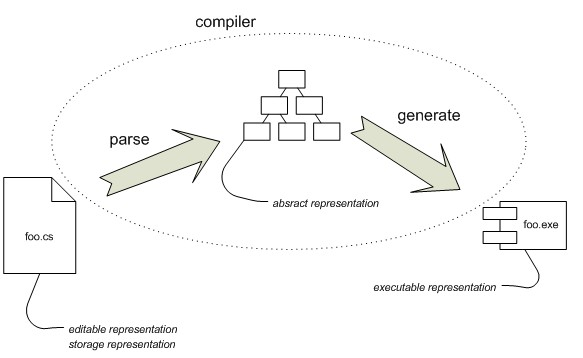
\includegraphics[width=0.8\textwidth]{chapters/fundamentacao/imagens/parsing.jpg}}

\par\medskip\textbf{Fonte:} \citeonline{martinfowlerprojectionalediting}. \par\medskip
\end{figure}


\newpage
No caso da abordagem projecional, utiliza-se editores gráficos para manipular diretamente as definições do sistema, ou seja, edita-se a representação abstrata, de modo que o programador possa modificar as definições mantidas no modelo. Nesse caso, o executável é produzido por uma série de projeções e transformações a partir desta representação abstrata (Figura \ref{fig:abordagemprojectional}).


\begin{figure}[ht!]
\centering

\caption{\textmd{Abordagem projecional}}
\label{fig:abordagemprojectional}
\fcolorbox{gray}{white}{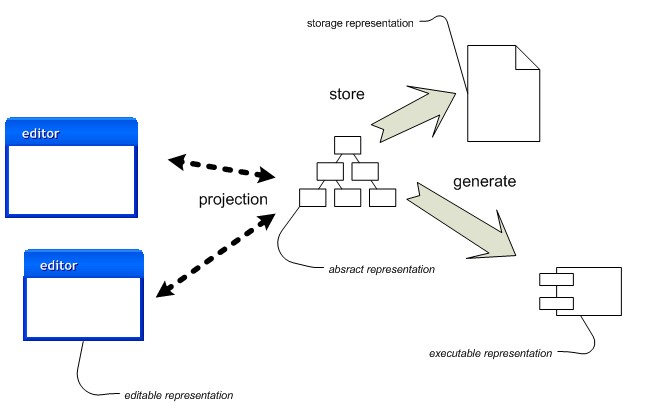
\includegraphics[width=0.8\textwidth]{chapters/fundamentacao/imagens/projectional.jpg}}

\par\medskip\textbf{Fonte:} \cite{martinfowlerprojectionalediting} \par\medskip
\end{figure}

Na Subseção \ref{exemplosferramentasdsl} são apresentados alguns exemplos de ferramentas de criação de \gls{DSL}s.

\newpage
\subsection{Exemplos de ferramentas}
\label{exemplosferramentasdsl}

\citeonline{fowler2005language}, apresenta em seu texto, a \textit{Intentional Software} como a precursora das ferramentas de criação de linguagens, foi desenvolvida por \textit{Charles Simonyi} no setor de pesquisa \textit{Microsoft Research}. 

Essa ferramenta permite a criação e edição de código de domínio, o qual é criado por meio da definição de um esquema de domínio pelo \textit{Domain Expert} com apoio dos desenvolvedores, para então ser construído um gerador de código que resulta na aplicação final \cite{simonyi2006intentional}. 

A ferramenta utiliza uma representação de domínio em formato de árvore de intenções, que é apresentada ao usuário em diferentes formas de visualização e edição, a Figura \ref{fig:intentional} mostra a árvore de intenção para uma instrução matemática simples.

\begin{figure}[h!]
\centering

\caption{\textmd{Árvore de intenção no \textit{Intentional Software}}}
\label{fig:intentional}
\fcolorbox{gray}{white}{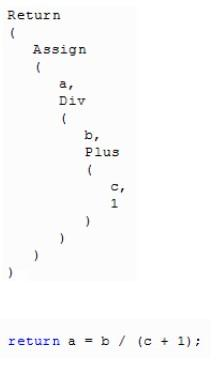
\includegraphics[width=0.4\textwidth]{chapters/fundamentacao/imagens/intentional.jpg}}

\par\medskip\textbf{Fonte:} \cite{simonyi2006intentional} \par\medskip
\end{figure}


Outra ferramenta de abordagem projecional é a \gls{MPS}, de código aberto sob a licença Apache 2.0 e é desenvolvida pela \textit{JetBrains}. Ela se baseia em definição de linguagens por meio de representação de texto estruturado, e possui uma série de recursos sofisticados de edição e ferramentas de navegação. 

Segundo \citeonline{dslengineering}, a \gls{MPS} suporta notações mistas (textuais, simbólicas, tabulares, gráficas) e uma ampla variedade de recursos de composição de idiomas. Ela define a linguagem por meio de \textit{Concepts} que são elementos para criação da sintaxe abstrata (Figura \ref{fig:mpsconceitos}), e esses conceitos são atrelados a um editor, o qual define as regras de projeção por meio de uma lista de células, que juntas definem a estrutura desejada para a sintaxe do conceito (Figura \ref{fig:mpseditor}).

\begin{figure}[h!]
\centering

\caption{\textmd{MPS definição de Conceitos}}
\label{fig:mpsconceitos}
\fcolorbox{gray}{white}{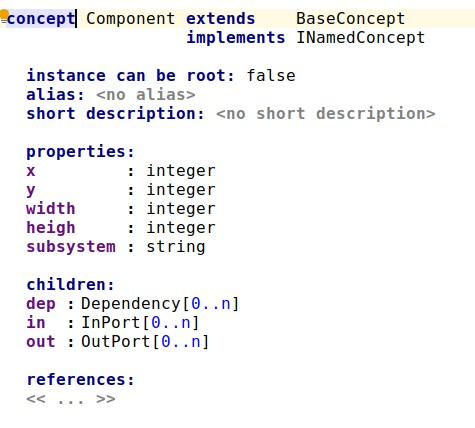
\includegraphics[width=\textwidth]{chapters/fundamentacao/imagens/mpsconceitos.jpg}}

\par\medskip\textbf{Fonte:} JetBrains (2018). \par\medskip
\end{figure}


\begin{figure}[ht!]
\centering

\caption{\textmd{MPS editor - sintaxe abstrata}}
\label{fig:mpseditor}
\fcolorbox{gray}{white}{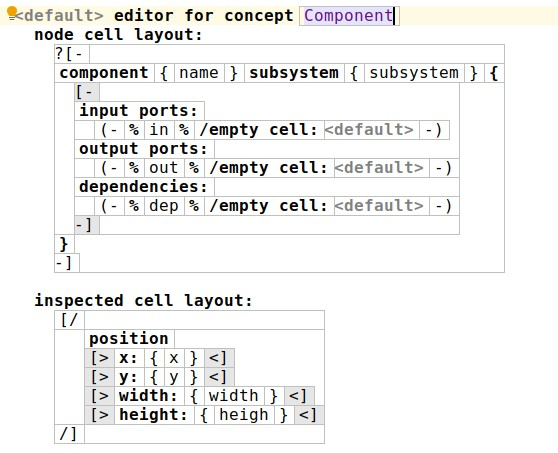
\includegraphics[width=0.98\textwidth]{chapters/fundamentacao/imagens/mpseditor.jpg}}

\par\medskip\textbf{Fonte:} JetBrains (2018). \par\medskip
\end{figure}


\newpage


Como alternativa às ferramentas projecionais, existem ferramentas que geram o \textit{parser} a partir da gramática, nesse caso, as regras da linguagem são expressadas em notação baseada em \gls{BNF}. As ferramentas Xtext e Spoofax são casos de ambientes nos quais é possível construir \gls{DSL}s por meio desse tipo de abordagem, a seguir são listados alguns exemplos nessas ferramentas.


\citeonline{eysholdt2010xtext}, descreve a ferramenta Xtext, como um \textit{framework} que permite o rápido desenvolvimento de ferramental de suporte às linguagens textuais, podendo atender desde linguagens menores como \gls{DSL}s, até linguagens completas \gls{GPL}s. Ela utiliza o core do \gls{EMF} para criar a \GLS{AST} a partir de uma especificação de gramática. 

Na Figura \ref{fig:xtextgramatica} é possível verificar a definição da gramática de uma linguagem específica para modelagem de entidades, de forma similar ao que existe em alguns \textit{frameworks} de programação, como Rails e Grails. O resultado é apresentado na Figura \ref{fig:xtextprograma}, na qual observa-se a utilização de recursos do Xtext no momento da codificação de um novo programa nessa linguagem.

\begin{figure}[ht!]
\centering

\caption{\textmd{Exemplo de definição de gramática Xtext}}
\label{fig:xtextgramatica}
\fcolorbox{gray}{white}{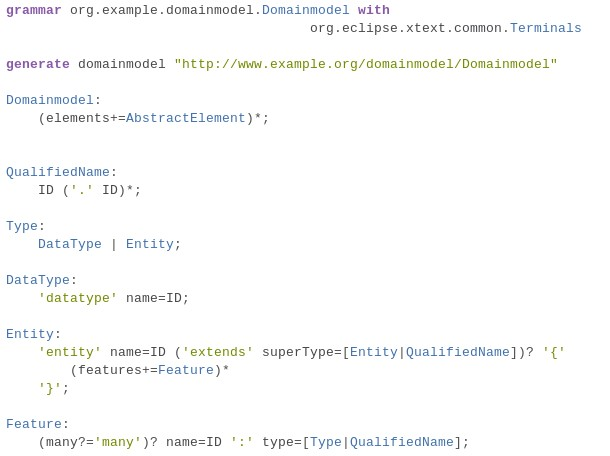
\includegraphics[width=0.9\textwidth]{chapters/fundamentacao/imagens/xtextgramatica.jpg}}

\par\medskip\textbf{Fonte:} \citeonline{xtextsite}. \par\medskip
\end{figure}


\begin{figure}[h!]
\centering

\caption{\textmd{Exemplo de uso da linguagem de entidades}}
\label{fig:xtextprograma}
\fcolorbox{gray}{white}{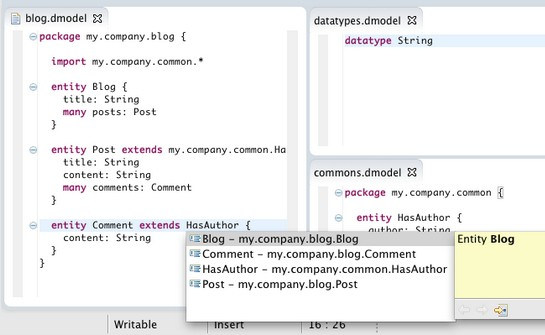
\includegraphics[width=0.9\textwidth]{chapters/fundamentacao/imagens/xtextprograma.jpg}}

\par\medskip\textbf{Fonte:} \citeonline{xtextsite}. \par\medskip
\end{figure}


\newpage
Por fim, a ferramenta \textit{Spoofax} utiliza o formato \gls{SDF} para descrição da sintaxe da linguagem, sendo um ambiente integrado de especificação de linguagens, com suporte e \textit{plugins} para a \gls{IDE} Eclipse. 

Um exemplo de definição de gramática em formato \gls{SDF} pode ser observado na Figura \ref{fig:spoofaxgramatica}. No canto esquerdo da imagem são definidas as regras da sintaxe, para uma linguagem de entidades similar a que foi utilizada no exemplo do Xtext. 

\begin{figure}[h!]
\centering

\caption{\textmd{Definição de gramática no Spoofax}}
\label{fig:spoofaxgramatica}
\fcolorbox{gray}{white}{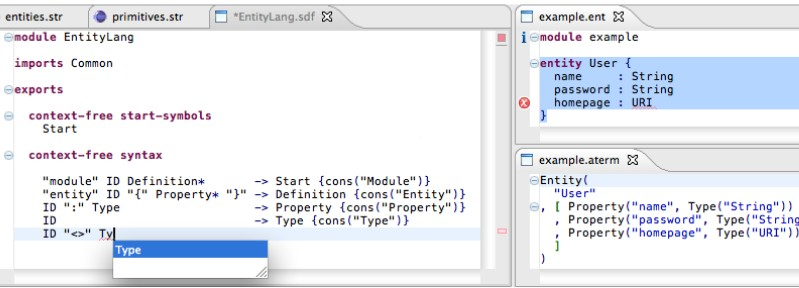
\includegraphics[width=0.9\textwidth]{chapters/fundamentacao/imagens/spoofaxgramatica.jpg}}

\par\medskip\textbf{Fonte:} \cite{kats2010spoofax} \par\medskip
\end{figure}



Segundo \citeonline{kats2010spoofax}, os seus editores permitem verificar e destacar erros por linha, validar tipos de dados da linguagem, resolução de referências, recursos de ajuda conforme contexto e até completar ou sugerir opções de código para o usuário da linguagem (Figura \ref{fig:spoofaxeditor}). 

\begin{figure}[h!]
\centering

\caption{\textmd{Recursos do editor Spoofax}}
\label{fig:spoofaxeditor}
\fcolorbox{gray}{white}{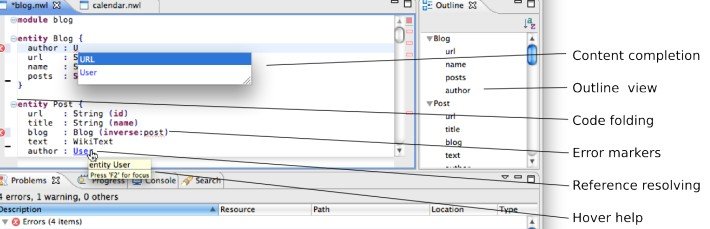
\includegraphics[width=\textwidth]{chapters/fundamentacao/imagens/spoofaxeditor.jpg}}

\par\medskip\textbf{Fonte:} \cite{kats2010spoofax} \par\medskip
\end{figure}


A fim de criar a linguagem de domínio proposta pelo presente trabalho, será necessário definir entre uma dessas ferramentas. Na Seção \ref{justificativamps} é apresentada a justificativa da escolha do \gls{MPS} como ferramenta para implementação da linguagem de especificação de regras de classificação pelo sistema de cotas.